\newpage
\begin{center}
{\Large{\textbf{Appendix}}}
\end{center}

\begin{appendix}
\section{Expression for $K^{(d)}$}\label{sec:kd}
The $K^{(d)}$ matrix is computed by the recursion in \eqref{eq:ntkold}.
\begin{align}\label{eq:ntkold}
&\tilde{K}^{(1)}(s,s')=\Sigma^{(1)}(s,s')=\Sigma(s,s'), M^{(l)}_{ss'}=\left[\begin{matrix}\Sigma^{(l)}(s,s) & \Sigma^{(l)}(s,s')\\ \Sigma^{(l)}(s',s) & \Sigma^{(l)}(s',s')\end{matrix}\right]\in \R^2,\nn\\
&\Sigma^{(l+1)}(s,s')= 2\cdot\mathbb{E}_{(q,q')\sim N(0,M_{ss'}^{(l)})} \left[\chi(q)\chi(q')\right], \hat{\Sigma}^{(l+1)}(s,s')= 2\cdot\mathbb{E}_{(q,q')\sim N(0,M_{ss'}^{(l)})}\left[\partial\chi(q)\partial{\chi}(q')\right],\nn\\
&\tilde{K}^{(l+1)}=\tilde{K}^{(l)}\odot \hat{\Sigma}^{(l+1)}+\Sigma^{(l+1)}, K^{(d)}=\left(\tilde{K}^{(d)}+\Sigma^{(d)}\right)/2
\end{align}
where $s,s'\in[n]$ are two input examples in the dataset, $\Sigma$ is the data Gram matrix, $\partial{\chi}$ stands for the derivative of the activation function with respect to the pre-activation input, $N(0,M)$ stands for the mean-zero Gaussian distribution with co-variance matrix $M$.



\section{Proofs of technical results}
\textbf{Proof of \Cref{prop:basic}}
\begin{proof}
We know that $e_t=(e_t(s),s\in[n])\in\R^n$, and $e_t(s)=\hat{y}_{\Theta_t}(x_s)-y(s)$. Now
\begin{align} 
L_{\Theta_t}&=\frac{1}2\sum_{s'=1}^n(\hat{y}_{\Theta_t}-y)^2\nn\\
&=\frac{1}2\sum_{s'=1}^n e_t^2\nn\\
\nabla_{\Theta} L_{\Theta_t}&= \sum_{s'=1}^n\nabla_{\Theta} \hat{y}_{\Theta_t}(x_{s'})e_t(s')\nn\\
\label{eq:above1} \nabla_{\Theta} L_{\Theta_t}&= \sum_{s'=1}^n \psi_{x_{s'},\Theta_t}e_t(s')
\end{align}
For gradient descent, $\dot{\Theta}_t=-\nabla_{\Theta} L_{\Theta_t}$, from \eqref{eq:above1} it follows that 
\begin{align}
\dot{\Theta}_t=-\sum_{s'=1}^n \psi_{x_{s'},\Theta_t}e_t(s')
\end{align}
Now $\dot{e}_t=\dot{\hat{y}}_{\Theta_t}$, and expanding $\dot{\hat{y}}_{\Theta_t}(x_s)$ for some $s\in[n]$, we have:
\begin{align}
\dot{\hat{y}}_{\Theta_t}(x_s)&=\frac{d \hat{y}_{\Theta_t}(x_s)}{d t}\nn\\
&=\sum_{\theta\in\Theta}\frac{d \hat{y}_{\Theta_t}(x_s)}{d \theta}\frac{d \theta_t}{dt},\,\text{by expressing this summation as a dot product we obtain} \nn\\
\dot{\hat{y}}_{\Theta_t}(x_s)&=\ip{\psi_{x_s,\Theta_t},\dot{\Theta}_t}
\end{align}
We now use that fact that $\Theta_t$ is updated by gradient descent
\begin{align}
\dot{\hat{y}}_{\Theta_t}(x_s)&=-\ip{\psi_{x_s,\Theta_t},\sum_{s'=1}^n \psi_{x_{s'},\Theta_t}e_t(s')}\nn\\
&=-\sum_{s'=1}^n K_{\Theta_t}(s,s')e_t(s')
\end{align}
The proof is complete by recalling that $\hat{y}_{\Theta_t}=(\hat{y}_{\Theta_t}(x_s),s\in[n])$, and $\dot{e}_t=\dot{\hat{y}}_{\Theta_t}$.
\end{proof}


\textbf{Proof of \Cref{prop:zero}}
\begin{proof}
Let $x\in\R^{\din}$ be the input to the DNN and $\hat{y}_{\Theta}(x)$ be its output. The output can be written in terms of the final hidden layer output as:
\begin{align}
\hat{y}_{\Theta}(x)&=\sum_{j_{d-1}=1}^w\Theta(1, j_{d-1},d) \cdot z_{x,\Theta}(j_{d-1},d-1)\nn\\
\label{lastlayer}&=\sum_{j_{d-1}=1}^w\Theta(1, j_{d-1},d) \cdot G_{x\Theta}(j_{d-1},d-1)\cdot q_{x,\Theta}(j_{d-1},d-1)
\end{align}
Now $q_{x,\Theta}(j_{d-1},d-1)$ for a fixed $j_{d-1}$ can again be expanded as
\begin{align}
q_{x,\Theta}(j_{d-1},d-1)&= \sum_{j_{d-2}=1}^w \Theta(j_{d-1},j_{d-2},d-1) \cdot z_{x,\Theta}(j_{d-2},d-2)\nn\\
\label{onebefore}&=\sum_{j_{d-2}=1}^w \Theta(j_{d-1},j_{d-2},d-1) \cdot G_{x,\Theta}(j_{d-2},d-2)\cdot q_{x,\Theta}(j_{d-2},d-2)
\end{align}
Now plugging in \eqref{onebefore} in the expression in \eqref{lastlayer}, we have
\begin{align}
\hat{y}_{\Theta}(x)&=\sum_{j_{d-1}=1}^w\Theta(1, j_{d-1},d)\cdot G_{x\Theta}(j_{d-1},d-1)\Bigg(\sum_{j_{d-2}=1}^w \Theta(j_{d-1},j_{d-2},d-1)\nn\\ &\hspace{15pt}\cdot G_{x,\Theta}(j_{d-2},d-2)\cdot q_{x,\Theta}(j_{d-2},d-2)\Bigg)\nn\\
&=\sum_{j_{d-1}, j_{d-2}\in[w]} G_{x,\Theta}(j_{d-1},d-1)\cdot G_{x,\Theta}(j_{d-2},d-2)\cdot\Theta(1, j_{d-1},d)\nn\\&\cdot \Theta(j_{d-1},j_{d-2},d-1)\cdot q_{x,\Theta}(j_{d-2},d-2)\nn\\
\end{align}
By expanding $q$'s for all the previous layers till the input layer we have
\begin{align}
\hat{y}_{\Theta}(x)=\sum_{j_{d}=1, j_{d-1},\ldots,j_{1}\in[w], j\in[\din]} x(j) \Pi_{l=1}^{d-1}G_{x,\Theta}(j_{l},l) \Pi_{l=1}^{d}\Theta(j_l, j_{l-1}, l) \nn
\end{align}
\end{proof}

\textbf{Proof of \Cref{lm:npk}}
\begin{proof}
\begin{align}
\ip{\phi_{x_s,\Theta},\phi_{x_{s'},\Theta}}&=\sum_{p\in[P]}x_s(\I_0(p))x_{s'}(\I_0(p))A_{\Theta}(x_s,p)A_{\Theta}(x_{s'},p)\nn\\
&=\sum_{i=1}^{\din}x_s(i)x_{s'}(i)\Lambda_{\Theta}(s,s')\nn\\
&=\ip{x_s,x_{s'}}\cdot\Lambda_{\Theta}(s,s')
\end{align}
\end{proof}

    \textbf{Proof of \Cref{prop:ntknew}}
\begin{proof}
Let $\Psi_{\Theta}=(\psi_{x_s,\Theta},s\in[n])\in\R^{\dnet\times n}$ be the NTF matrix, then the NTK matrix is given by $K_{\Theta_t}=\Psi^\top_{\Theta_t}\Psi_{\Theta_t}$. Note that, $\hat{y}_{\Theta}(x_s)=\ip{\phi_{x_s,\Theta},v_{\Theta}}=\ip{v_{\Theta},\phi_{x_s,\Theta}}=v^\top_{\Theta}\phi_{x_s,\Theta}$. Now $\psi_{x_{s},\Theta}=\nabla_{\Theta} v_{\Theta}\phi_{x_s,\Theta}$, and hence $\Psi=\nabla_{\Theta} v_{\Theta}\Phi_{\Theta}$. Hence, $K_{\Theta_t}=\Psi^\top_{\Theta_t}\Psi_{\Theta_t}=\Phi^\top_{\Theta}(\nabla_{\Theta} v_{\Theta})^\top (\nabla_{\Theta} v_{\Theta})\Phi_{\Theta}=\Phi^\top_{\Theta}\V_{\Theta}\Phi_{\Theta}$.
\end{proof}

\textbf{Proof of \Cref{prop:dnnhard}}

\begin{proof}
Follows in a similar manner as the proof of \Cref{prop:basic}.
\end{proof}

\textbf{Proof of {\Cref{prop:condition}}}
\begin{proof}
$\rho_{\min}(K_{\Theta})=\underset{\norm{x}_2=1}{\underset{x\in \R^n}\min}x^\top K_{\Theta} x$. Let $x'\in\R^n$ such that $\norm{x'}_2=1$ and $\rho_{\min}(H_{\Theta})={x'}^\top H_{\Theta} x'$. Now, $\rho_{\min}(K_{\Theta})\leq {x'}^\top K_{\Theta} x'$. 
Let $y'=\Phi x'$, then we have, $\rho_{\min}(K_{\Theta})\leq {y'}^\top \V_{\Theta}y'$. Hence $\rho_{\min}(K_{\Theta})\leq \norm{y'}^2_2 \rho_{\max}(\V_{\Theta})$. Proof is complete by noting that $\norm{y'}^2_2={x'}^\top \Phi^\top_{\Theta}\Phi_{\Theta}x'= \rho_{\min}(H_{\Theta})$.
\end{proof}


\textbf{Proof of \Cref{prop:dgn}}

\begin{proof}
Follows in a similar manner as proof of \Cref{prop:basic}.
\end{proof}

\subsection{Proof of \Cref{th:main}}
\subsubsection{Calculation of $\E{K^\text{v}_{\Tdgn_0}}$}

\begin{proposition}
Let $\tv\in\Tv$ be a weight in layer $l_{\tv}$, and let $p$ be a path that passes through $\tv$. Then 
\begin{align}
\partial_{\tv} v_{\Tv}(p) =& \Pi_{l=1,l\neq l_{\tv}}^{d} \Theta(\I_{l}(p),\I_{l-1}(p),l )
\end{align}
\end{proposition}
\begin{proof}
Proof follows by noting that $v_{\Tv}(p)=\Pi_{l=1}^{d}\Theta(\I_l(p),\I_{l-1}(p),l)$.
\end{proof}


\begin{lemma}\label{lm:dot}
Let $\varphi_{p,\Theta}$ be as in \Cref{def:npvgrad}, under the assumption in ~\Cref{th:main}, for paths $p_1,p_2\in [P], p_1\neq p_2$, at initialisation we have (i) $\E{\ip{\varphi_{p_1,\Tv_0}, \varphi_{p_2,\Tv_0}}}= 0$, (ii) ${\ip{\varphi_{p_1,\Tv_0}, \varphi_{p_1,\Tv_0}}}= d\cdot \sigma^{2(d-1)}$.
\end{lemma}

\begin{proof}
\begin{align*}
\ip{\varphi_{p_1,\Tv_0}, \varphi_{p_2,\Tv_0}}= \sum_{\tv\in \Tv} \partial_{\tv}v_{\Tv_0}(p_1) \partial_{\tv}v_{\Tv_0}(p_2)
\end{align*}
Let $\tv\in\Tv$ be an arbitrary weight. If either $p_1$ or $p_2$ does not pass through $\tv$, then it follows that $\partial_{\tv} v_{\Tv_0}(p_1) \partial_{\tv} v_{\Tv_0}(p_2)=0$. Let us consider the the case when $p_1,p_2$ pass through $\tv$ and without of loss of generality let $\tv$ belong to layer $l_{\tv}\in[d]$. 
  we have
\begin{align*}
&\E{\partial_{\tv}v_{\Tv_0}(p_1)\partial_{\tv}v_{\Tv_0}(p_2)}\\
&=\E{\underset{l\neq l_{\tv}}{\underset{l=1}{\overset{d}{\Pi}}} \Bigg(\Tv_0(\I_{l} (p_1),  \I_{l-1}(p_1),l) \Tv_0(\I_{l}(p_2),\I_{l-1} (p_2),l) \Bigg)}\\
&=\underset{l\neq l_{\tv}}{\underset{l=1}{\overset{d}{\Pi}}}\E{\Tv_0(\I_{l}(p_1),\I_{l-1}(p_1),l)\Tv_0(\I_{l}(p_2),\I_{l-1}(p_2),l)}
\end{align*}
where the $\E{\cdot}$ moved inside the product because at initialisation the weights (of different layers) are independent of each other.
Since $p_1\neq p_2$, there exist a layer $\tilde{l}\in[d],\tilde{l}\neq l_{\tv}$ such that they do not pass through the same weight in layer $\tilde{l}$, i.e., $\Tv_0(\I_{\tilde{l}}(p_1),\I_{\tilde{l}-1}(p_1),\tilde{l},)$ and $\Tv_0(\I_{\tilde{l}}(p_2),\I_{\tilde{l}-1}(p_2),\tilde{l})$ are distinct weights. Using this fact,  we have 
\begin{align*}
&\E{\partial_{\tv}v_{\Tv_0}(p_1)\partial_{\tv}v_{\Tv_0}(p_2)}\\
=&\Bigg(\underset{l\neq l_{\tv},\tilde{l}}{\underset{l=1}{\overset{d}{\Pi}}}\E{\Tv_0(\I_l(p_1), \I_{l-1}(p_1),l)\Tv_0(\I_{l}(p_2),\I_{l-1}(p_2),l)}\Bigg)\\
&\cdot\Bigg(\E{\Tv_0(\I_{\tilde{l}}(p_1),\I_{\tilde{l}-1} (p_1),\tilde{l})}\E{\Tv_0(\I_{\tilde{l}}(p_2), \I_{\tilde{l}-1 }(p_2),\tilde{l})}\Bigg)\\
=&0
\end{align*}

The proof of (ii) is complete by noting that a given path $p_1$ pass through only `$d$' weights, and hence $\sum_{\tv\in\Tv} \partial_{\tv}v_{\Tv_0}(p_1) \partial_{\tv}v_{\Tv_0}(p_1)$ has `$d$' non-zero terms, and the fact that at initialisation we have 
\begin{align*}
&\partial_{\tv}v_{\Tv_0}(p_1) \partial_{\tv}v_{\Tv_0}(p_1) \\
&=\underset{l\neq l_{\tv}}{\underset{l=1}{\overset{d}{\Pi}}} [\Tv_0(\I_{l}(p),\I_{l-1}(p),l)]^2\\
&=\sigma^{2(d-1)}
\end{align*}
\end{proof}



\begin{theorem}\label{th:exp}
 $\E{K^{\text{v}}_{\Tdgn_0}}=d\cdot\sigma^{2(d-1)} \cdot H_{\text{FNPF}}$. 
\end{theorem}
\begin{proof}
Let $\Phi_{\text{FNPF}}=\Phi_{\Tf_0}=\left(\phi_{x_s,\Tf_0}, s\in[n]\right)\in\R^{P\times n}$ be the NPF matrix. 
\begin{align*}
\E{K^{\text{v}}_{\Tdgn_0}}&=\E{\Phi^\top_{\text{FNPF}} \V_{\Tv_0} \Phi_{\text{FNPF}}}\\
&=\E{\Phi^\top_{\text{FNPF}} (\nabla_{\Tv}v_{\Tv_0})^\top (\nabla_{\Tv}v_{\Tv_0}) \Phi_{\text{FNPF}}}\\
&=\Phi^\top_{\text{FNPF}}\left( \E{(\nabla_{\Tv}v_{\Tv_0})^\top (\nabla_{\Tv}v_{\Tv_0})}\right)\Phi_{\text{FNPF}}\\
&\stackrel{(a)}=d\cdot\sigma^{2(d-1)} \cdot\left(\Phi^\top_{\text{FNPF}}\Phi_{\text{FNPF}}\right)\\
&=d\cdot\sigma^{2(d-1)} \cdot H_{\text{FNPF}}
\end{align*}
Here, $(a)$ follows from  \Cref{lm:dot}, i.e., $\E{(\nabla_{\Tv}v_{\Tv_0})^\top (\nabla_{\Tv}v_{\Tv_0})}= d\cdot\sigma^{2(d-1)}\cdot I_{P\times P}$, where $I_{P\times P}$ is a ${P\times P}$ identity matrix.
\end{proof}

\subsubsection{Calculation of $Var\left[K^\text{v}_{\Tdgn_0}\right]$}

\input{varproof}

\textbf{Proof of\Cref{th:main}}
\begin{proof} Follows from \Cref{th:exp} and \Cref{th:var}.
\end{proof}


\section{Applying \Cref{th:main} In Finite Width Case}\label{sec:finite}
In this section, we describe the technical step in applying \Cref{th:main} which requires $w\ra\infty$ to measure the information in the gates of a DNN  with finite width.  Since we are training only the value network in the FPNP mode of the DGN, it is possible to let the width of the value network alone go to $\infty$, while keeping the width of the feature network (which stores the fixed NPFs) finite. This is easily achieved by multiplying the width by a positive integer $m\in\Z_{+}$, and \emph{padding} the gates `$m$' times.
\begin{definition}
Define DGN${}^{(m)}$ to be the DGN whose feature network is of width $w$ and depth $d$, and whose value network  is a fully connected network of width $mw$ and depth $d$. The $mw(d-1)$ gating values are obtained by `padding' the $w(d-1)$gating values of the width `$w$', depth `$d$' feature network `$m$' times (see \Cref{fig:dgnpad}, \Cref{tb:dgnpad}). 
\end{definition}
\FloatBarrier
\begin{table}[h]
\centering
\begin{tabular}{|  l | l |}\hline
 Feature Network (NPF)& Value Network (NPV)\\
 $z^{\text{f}}_{x}(0)=x$ &$z^{\text{v}}_{x}(0)=x$ \\
$q^{\text{f}}_{x}(i,l)=\sum_{j} \Tf(i,j,l)\cdot z_{x}(j,l-1)$ & $q^{\text{v}}_{x}(i,l)=\sum_{j} \Tv(i,j,l)\cdot z^{\text{v}}_{x}(j,l-1)$\\
$z^{\text{f}}_{x}(i,l)= q^{\text{f}}_{x}(i,l)\cdot\mathbbm{1}_{\{q^{\text{f}}_{x}(i,l)>0\}}$& $z^{\text{v}}_{x}(i,l)= q^{\text{v}}_{x}(i,l)\cdot G_{x}(i,l)$ \\
 None &$\hat{y}_{{\Tdgn}^{(m)}}(x)= \sum_{j} \Tv(1,j,l)\cdot z^{\text{v}}_{x}(j,d-1)$\\\hline
\multicolumn{2}{|l|}{{Hard ReLU: $G_{x}(i,l)=\mathbbm{1}_{\{q^{\text{f}}_{x}(i,l)>0\}}$ or Soft-ReLU: $G_{x}(i,l)={1}/{\left(1+\exp(-\beta\cdot q^{\text{f}}_{x}(i,l)>0)\right)} $}}\\\hline
\end{tabular}
\caption{Deep Gated Network with padding. Here the gating values are padded, i.e., $ G_{x}(kw+i,l)=G_{x}(i,l),\forall k=0,1,\ldots,m-1, i\in[w]$. }
\label{tb:dgnpad}
\end{table}



\textbf{Remark:}  DGN${}^{(m)}$ has a total of $P^{(m)}=(mw)^{(d-1)}\din$ paths. Thus, the NPF and NPV are quantities in $\R^{P^{(m)}}$. In what follows, we denote the NPF matrix of DGN${}^{(m)}$ by $\Phi^{(m)}_{\Tf_0}\in\R^{P^{(m)}\times n}$, and use $H^{(m)}_{\text{FNPF}}=(\Phi^{(m)}_{\Tf_0})^\top \Phi^{(m)}_{\Tf_0}$. 

Before we proceed to state the version of \Cref{th:main} for DGN${}^{(m)}$, we will look at an equivalent definition for $\Lambda_{\Theta}$ (see \Cref{def:lambda}).
\begin{definition}\label{def:equilambda}
For input examples $s, s'\in[n]$ define 

$1.$ $\tau_{\Theta}(s,s',l)\stackrel{def}=\sum_{i=1}^w G_{x_s,\Theta}(i,l)G_{x_{s'},\Theta}(i,l)$ be the number of activations that are ``on'' for both inputs $s,s'\in[n]$ in layer $l\in[d-1]$.

$2.$ $\Lambda_{\Theta}(s,s')\stackrel{def}=\Pi_{l=1}^{d-1}\tau_{\Theta}(s,s',l)$.
\end{definition}

\FloatBarrier
\begin{figure}[h]
\centering
%\resizebox{\columnwidth}{\textheight}{
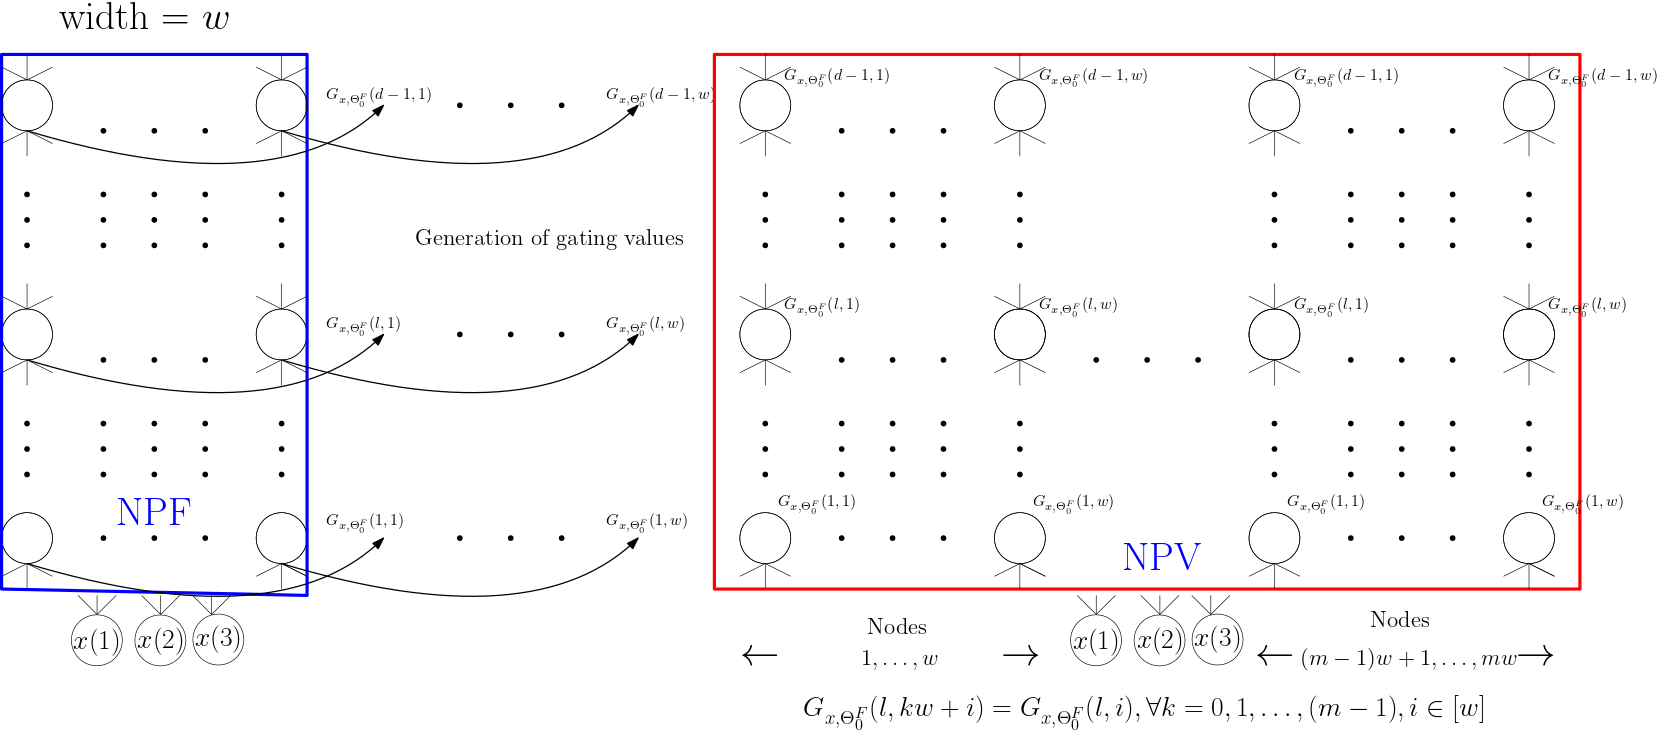
\includegraphics[scale=0.1]{figs/dgn-infty.png}
%}
\caption{DGN${}^{(m)}$ where the value network is of width $mw$ and depth $d$. The gates are derived by padding the gating values obtained from the feature network `$m$' times, i.e., $ G_{x}(kw+i,l)=G_{x}(i,l),\forall k=0,1,\ldots,m-1, i\in[w]$.}
\label{fig:dgnpad}
\end{figure}



\begin{corollary}[Corollary to \Cref{th:main}] Under the same assumptions as in \Cref{th:main} with $\sigma$ replaced by $\sigma_{(m)}=\sigma/\sqrt{m}$, as $m\ra\infty$, \begin{align*}K^{\text{v}}_{\Theta^{\text{DGN}^{(m)}}_0}\ra K^{(d)}_{\text{FNPF}} = d\cdot \sigma_{(m)}^{2(d-1)} H^{(m)}_{\text{FNPF}}= d\cdot \sigma^{2(d-1)} H_{\text{FNPF}}\end{align*}
\end{corollary}
\begin{proof}
Let $\Lambda^{(m)}_{\text{FNPF}}$ and $\tau^{(m)}_{\text{FNPF}}$ be quantities associated with DGN${}^{(m)}$. We know that  $H^{(m)}_{\text{FNFP}}=\Sigma\odot\Lambda^{(m)}_{\text{FNPF}}$. Dropping the subscript FNPF to avoid notational clutter, we have
\begin{align*}
\left(\sigma/\sqrt{m}\right)^{2(d-1)}\Lambda^{(m)}(s,s')&=\sigma^{2(d-1)}\frac{1}{m^{(d-1)}}\Pi_{l=1}^{d-1}\tau^{(m)}(s,s',l)\\
&=\sigma^{2(d-1)}\frac{1}{m^{(d-1)}}\Pi_{l=1}^{d-1}\left(m \tau(s,s',l)\right)\\
&=\sigma^{2(d-1)}\frac{1}{m^{(d-1)}}m^{(d-1)}\Pi_{l=1}^{d-1} \tau(s,s',l)\\
&=\sigma^{2(d-1)}\Pi_{l=1}^{d-1} \tau(s,s',l)\\
&=\sigma^{2(d-1)}\Lambda(s,s')
\end{align*}
\end{proof}


\section{DGN as a Lookup Table: Applying \Cref{th:main} to a pure memorisation task}\label{sec:mem}

In this section, we modify the DGN in \Cref{fig:dgn} into a memorisation network to solve a pure memorisation task. The objective of constructing the memorisation network is to understand the roles of depth and width in \Cref{th:main} in a simplified setting. In this setting, we show increasing depth till a point helps in training and increasing depth beyond it hurts training. 

\begin{definition}[Memorisation Network/Task]
Given a set of values $(y_s)_{s=1}^n\in  \R$, a memorisation network (with weights $\Theta\in\R^{\dnet}$) accepts $s\in[n]$ as its input and produces $\hat{y}_{\Theta}(s)\approx y_s$ as its output. The loss of the memorisation network is defined as $L_{\Theta}=\frac{1}{2}\sum_{s=1}^n (\hat{y}_{\Theta}(s)-y_s)^2$.
\end{definition}
\FloatBarrier
\begin{table}[h]
\centering
\begin{tabular}{| l |  l  |}\hline
Layer&  Memorisation Network\\\hline
Input  &$z_{\Theta}(0)=1$ \\
Pre-Activation & $q_{s,\Theta}(l)=\sum_{j}\Theta(i,j,l)\cdot z_{s,\Theta}(j,l-1)$\\
Hidden & $z_{s,\Theta}(i,l)=q_{s,\Theta}(i,l)\cdot G_{s}(i,l)$ \\
Final  Output & $\hat{y}_{\Theta}(s)=\sum_{j} \Theta(1,j,d) \cdot z_{s,\Theta}(j,d-1)$\\\hline
\end{tabular}
\caption{ Memorisation Network. The input is fixed and is equal to $1$. All the internal variables depend on the index $s$ and the parameter $\Theta$. The gating values $G_s(i,l)$ are external and independent variables.}
\label{tb:dgnmemo}
\end{table}

\textbf{Fixed Random Gating:} The memorisation network is described in \Cref{tb:dgnmemo}. In a memorisation network, the gates are \emph{fixed and random}, i.e., for each index $s\in[n]$, the gating values $G_{s}(i,l),\forall l\in[d-1], i\in[w] $ are sampled from $Ber(\mu), \mu\in(0,1)$ taking values in $\{0,1\}$,  and kept fixed throughout training. The input to the memorisation network is fixed as $1$, and since the gating is fixed and random there is a separate random sub-network to memorise each target $y_s\in\R$. The memorisation network can be used to memorise the targets  $(y_s)_{s=1}^n$ by training it using gradient descent by minimising the squared loss $L_{\Theta}$. In what follows, we let $K_0$ and $H_0$ to be the NTK and NPK of the memorisation network at initialisation.


\textbf{Performance of Memorisation Network:} From \Cref{prop:basic} we know that as $w\ra\infty$, the training error dynamics of the memorisation network follows:
\begin{align}
\dot{e}_t=-K_{0} e_t,
\end{align}
i.e., the spectral properties of $K_0$ (or $H_0$) dictates the rate of convergence of the training error to $0$. In the case of the memorisation network with fixed and random gates, we can calculate $\E{K_0}$ explicitly. 

\textbf{Spectrum of $H_0$:} The input Gram matrix $\Sigma$ is a $n\times n$ matrix with all entries equal to $1$ and its rank is equal to 1, and hence $H_0=\Lambda_0$. We can now calculate the properties of $\Lambda_0$. It is easy to check that $\mathbb{E}_{\mu}\left[\Lambda_0(s,s)\right]=(\mu w)^{(d-1)},\forall s\in[n]$ and $\mathbb{E}_{\mu}\left[\Lambda_0(s,s')\right]=(\mu^2 w)^{(d-1)},\forall s,s'\in[n]$.  For $\sigma=\sqrt{\frac{1}{\mu w}}$, and $\mathbb{E}_{\mu}\left[K_0(s,s)/d\right]=1$, and $\mathbb{E}_{\mu}\left[K_0(s,s')/d\right]=\mu^{(d-1)}$. 
\begin{figure}
\centering
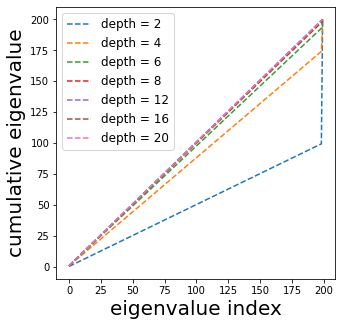
\includegraphics[scale=0.3]{figs/dgn-fra-ecdf-ideal-small.png}
\caption{Ideal spectrum of $\E{K_0}/d$ for a memorisation network for $n=200$.}
\label{fig:ideal-spectrum}
\end{figure}


\textbf{Why increasing depth till a point helps ?} 
We have:
%\comment{
\begin{align}\label{eq:mat}
\frac{\E{K_0}}{d}=\left[\begin{matrix}
1 &\mu^{d-1} &\ldots &\mu^{d-1} &\ldots\\ 
\ldots &1 &\ldots &\mu^{d-1} &\ldots\\ 
\ldots &\mu^{d-1} &\ldots &1 &\ldots \\
\ldots &\mu^{d-1} &\ldots &\mu^{d-1} &1\\ 
\end{matrix}\right]
\end{align}
%}
i.e., all the diagonal entries are $1$ and non-diagonal entries are $\mu^{d-1}$. Now, let $\rho_i\geq 0,i \in [n]$ be the eigenvalues of $\frac{\E{K_0}}{d}$, and let $\rho_{\max}$ and $\rho_{\min}$ be the largest and smallest eigenvalues.  One can easily show that $\rho_{\max}=1+(n-1)\mu^{d-1}$ and corresponds to the eigenvector with all entries as $1$, and $\rho_{\min}=(1-\mu^{d-1})$ repeats $(n-1)$ times,  which corresponds to eigenvectors given by $[0, 0, \ldots, \underbrace{1, -1}_{\text{$i$ and $i+1$}}, 0,0,\ldots, 0]^\top \in \R^n$ for $i=1,\ldots,n-1$. Note that as $d\ra\infty$, $\rho_{\max},\rho_{\min}\ra 1$.

\textbf{Why increasing depth beyond a point hurts?} 
As the depth increases the variance of the entries $K_0(s,s')$ deviates from its expected value $\E{K_0(s,s')}$. Thus the structure of the Gram matrix degrades from \eqref{eq:mat}, leading to smaller eigenvalues.
%\FloatBarrier
\begin{figure}
\resizebox{\textwidth}{!}{
\begin{tabular}{cccc}
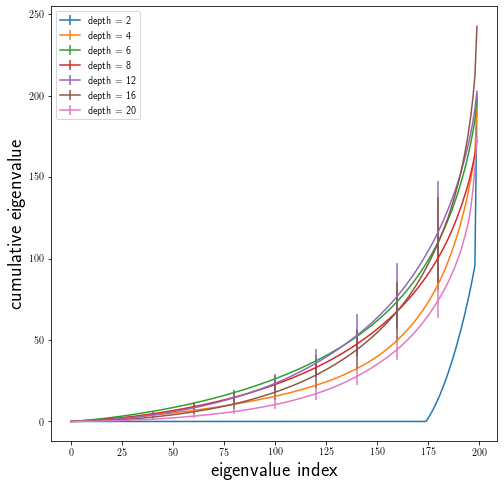
\includegraphics[scale=0.5]{figs/dgn-fra-ecdfbyd-w25.png}
&
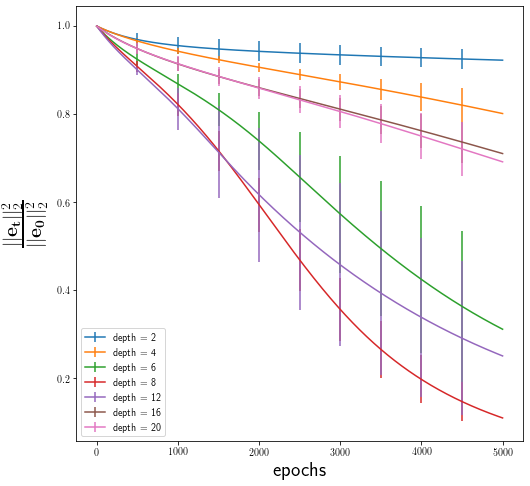
\includegraphics[scale=0.5]{figs/dgn-fra-conv-w25.png}
&
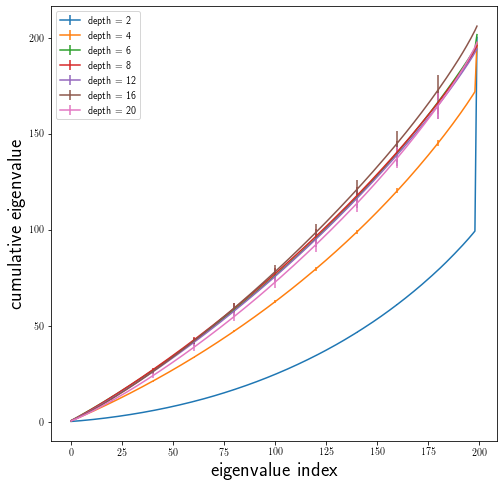
\includegraphics[scale=0.5]{figs/dgn-fra-ecdfbyd-w500.png}
&
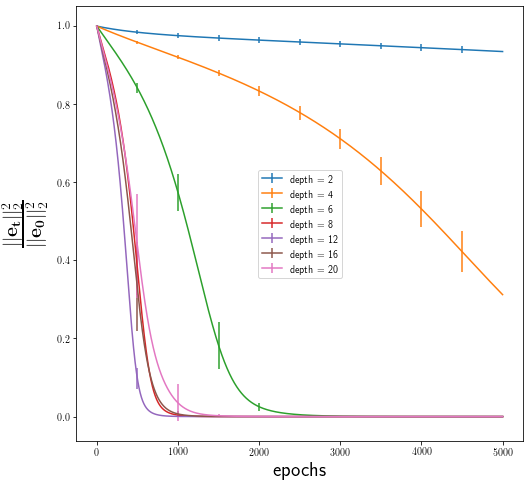
\includegraphics[scale=0.5]{figs/dgn-fra-conv-w500.png}
\end{tabular}
}
\caption{Shows the plots for the memorisation network with $\mu=\frac{1}{2}$ and $\sigma=\sqrt{\frac{2}{w}}$. The number of points to be memorised is $n=200$. The left most plot shows the e.c.d.f for $w=25$ and the second plot from the left shows the error dynamics during training for $w=25$. The second plot from the right shows the e.c.d.f for $w=500$ and the right most plot shows the error dynamics during training for $w=500$. All plots are averaged over $10$ runs.}
\label{fig:dgn-frg-gram-ecdf}
\end{figure}

\subsection{Experiment}
We set $n=200$, and $y_s\sim\text{Uniform}[-1,1]$. We look at the cumulative eigenvalue (e.c.d.f) obtained by first sorting the eigenvalues in ascending order then looking at their cumulative sum. The ideal behaviour (\Cref{fig:ideal-spectrum}) as predicted from theory is that for indices $k\in[n-1]$, the e.c.d.f should increase at a linear rate, i.e., the cumulative sum of the first $k$ indices is equal to $k(1-\mu^{d-1})$, and the difference between the last two indices is $1+(n-1)\mu^{d-1}$. In \Cref{fig:dgn-frg-gram-ecdf}, we plot the actual e.c.d.f for various depths $d=2,4,6,8,12,16,20$ and $w=25,500$ (first and third plots from the left in \Cref{fig:dgn-frg-gram-ecdf}). 

\textbf{Roles of depth and width:} In order to compare how the rate of convergence varies with the depth, we set the step-size $\alpha=\frac{0.1}{\rho_{\max}}$, $w=100$. We use the vanilla SGD-optimiser. Note the$ \frac{1}{\rho_{\max}}$ in the stepsize, ensures that the uniformity of maximum eigenvalue across all the instances, and the convergence should be limited by the smaller eigenvalues. We also look at the convergence rate of the ratio $\frac{\norm{e_t}^2_2}{\norm{e_0}^2_2}$. We notice that for $w=25$, increasing depth till $d=8$ improves the convergence, however increasing beyond $d=8$ worsens the convergence rate. For $w=500$, increasing the depth till $d=12$ improves convergence, and $d=16,20$ are worse than $d=12$.  %This matches with the depth phenomena observed in practical DNNs and also matches our theory.
\end{appendix}